\themaE
\graphicspath{{../../S09_Somme_des_angles_d_un_triangle/Images/}}

\chapter{Somme des angles\\d'un triangle}
\label{S09}

\renewcommand{\RedactionSomme}{La somme des angles du triangle $\NomTriangle$ fait \udeg{180} d'où :}


%%%%%%%%%%%%%%%%%%%%%%
%%%%%%%%%%%%%%%%%%%%%%
\begin{autoeval}
   \small
   \begin{enumerate}
      \item Il mobilise des connaissances sur des figures, des configurations pour déterminer des grandeurs géométriques (somme des angles d'un triangle).
   \end{enumerate}
\end{autoeval}

\begin{prerequis}
   \begin{itemize}
      \item Somme des angles d'un triangle.
      \item Mener des raisonnements et s'initier à la démonstration en utilisant les propriétés d'une figure.
   \end{itemize}
\end{prerequis}

\vfill

\begin{debat}[Débat : géométrie euclidienne VS géométrie sphérique]
   \og Un ours part de sa caverne et parcourt 10 km vers le sud, puis 10 km vers l'est et enfin 10 km vers le nord. Il se retrouve alors juste devant l'entrée de sa caverne. Quelle est la couleur de l'ours ? \fg \\
   La {\bf géométrie sphérique} n'a pas les même propriétés que la {\bf géométrie euclidienne} utilisée au collège et au lycée. Cette dernière est la géométrie initiée par {\it Euclide}, mathématicien grec né vers 330 av. J.-C., il est connu pour avoir recensé une grande partie des mathématiques de l'époque dans ses {\it Éléments} : une série de treize livres utilisée pendant près de 2\,000 ans qui fut l'ouvrage le plus édité au monde après la Bible. \\
   \begin{minipage}{5cm}
      \begin{pspicture}(-1,0.5)(4,3)
         \pspolygon[linecolor=C1](1,0)(4,0)(3,3.25)
      \end{pspicture}
   \end{minipage}
   \textcolor{B1}{
   \begin{minipage}{5cm}
      \flushright Un triangle \og sphérique \fg{} $\Longrightarrow$ \\
      \flushleft $\Longleftarrow$ Un triangle \og plat \fg \\     
   \end{minipage}}
   \begin{minipage}{5cm}
      \Reperage[Espace,Sphere,EchelleEspace=60,AnglePhi=30]{70/90/A,0/90/B}
   \end{minipage} 
  \bigskip
   \begin{cadre}[B2][J4]
      \begin{center}
         Vidéo : \href{https://leblob.fr/videos/les-triangles-et-astronomie}{\bf Les triangles et l'astronomie}, site Internet {\it Le blob}, épisode de la série {\it Math.ing}.
      \end{center}
   \end{cadre}
\end{debat}


%%%%%%%%%%%%%%%%%%%%%%%%%%%%%%%
%%%%%%%%%%%%%%%%%%%%%%%%%%%%%%%
\activites

\begin{activite}[Des angles mouvants]
   {\bf Objectif :} faire découvrir la propriété de la somme des angles d'un triangle.
   \begin{QCM}
   \partie[construction du triangle]
      \begin{enumerate}
         \item Sur une feuille, tracer un triangle ABC quelconque puis le découper.
         \item Colorier les trois angles de trois couleurs différentes des deux côtés du triangle (une couleur par angle). \\
         {\psset{unit=1.2}
         \begin{pspicture}(-2,0.2)(10,5.8)
            \rput(8.3,4.8){$\leftarrow$ colorier des deux côtés}
            \psline[linestyle=dashed](6,5)(6,1)(6.3,1)
            \psframe(6,1)(6.25,1.25)
            \pswedge[fillstyle=solid,fillcolor=B1,linecolor=B1](1,1){1}{0}{38.5}
            \pswedge[fillstyle=solid,fillcolor=A1,linecolor=A1](6,5){1}{218.8}{306.8}
            \pswedge[fillstyle=solid,fillcolor=J1,linecolor=J1](9,1){1}{127}{180}
            \pspolygon(1,1)(9,1)(6,5)
            \rput(0.7,1){B}
            \rput(9.3,1){C}
            \rput(6,5.3){A}
            \rput(6,0.7){H}     
         \end{pspicture}}
         \item Tracer la hauteur issue du sommet A et nommer le pied de cette hauteur H.
         \item Plier le triangle ABC de manière à placer le point A sur le point H.
         \item Plier le triangle ABC de manière à placer le point B sur le point H.
         \item Plier le triangle ABC de manière à placer le point C sur le point H.
      \end{enumerate}
   \partie[observations]
      \begin{enumerate}
         \item Que forment les trois angles obtenus en H ? \\ [5mm]
         \mbox{} \pointilles \\
         \item Formuler cette observation en utilisant les angles $\widehat{\text A}, \widehat{\text B}$ et $\widehat{\text C}$. \\ [5mm]
         \mbox{} \pointilles \\
         \item Formuler cette observation par une phrase simple et générale sans utiliser le nom des angles. \\ [5mm]
         \mbox{} \pointilles \\ [5mm]
         \mbox{} \pointilles \\
      \end{enumerate}
   \end{QCM}
\end{activite}


%%%%%%%%%%%%%%%%%%%%%%%%%%%%%%%
%%%%%%%%%%%%%%%%%%%%%%%%%%%%%%%
\cours 


%%%%%%%%%%%%%%%%%%%%%%
\section{Somme des angles dans un triangle}

\begin{propriete}
   Dans un triangle, la somme de la mesure de ses trois angles est égale à \udeg{180}.
\end{propriete}

\medskip

Par conséquent, pour qu'un triangle soit constructible, il est nécessaire que la somme de ses angles fasse \udeg{180}.
   
\begin{center}
   {\psset{unit=1}
   \begin{pspicture}(-1,0.5)(9,5.6)
      \pswedge[fillstyle=solid,fillcolor=B1,linecolor=B1](1,1){1}{0}{38.5}
      \pswedge[fillstyle=solid,fillcolor=A1,linecolor=A1](6,5){1}{218.8}{306.8}
      \pswedge[fillstyle=solid,fillcolor=J1,linecolor=J1](9,1){1}{127}{180}
      \pspolygon(1,1)(9,1)(6,5)
      \rput(0.7,1){B}
      \rput(9.3,1){C}
      \rput(6,5.3){A} 
      \rput(5.5,2.5){$\widehat{A}+\widehat{B}+\widehat{C} =\udeg{180}$}
      \pswedge[fillstyle=solid,fillcolor=B1,linecolor=B1](0,3){1}{141}{180}
      \pswedge[fillstyle=solid,fillcolor=A1,linecolor=A1](0,3){1}{53}{141}
      \pswedge[fillstyle=solid,fillcolor=J1,linecolor=J1](0,3){1}{0}{53}
      \rput(-0.7,3.2){\white B}
      \rput(-0.1,3.6){\white A}
      \rput(0.6,3.3){\white C}
   \end{pspicture}}
\end{center}

\begin{exemple}
   \SommeAngles[FigureSeule,Rectangle,Echelle=10mm]{CBA}{}{55} \\ [1mm]
   Calculer la mesure de l'angle $\widehat{BCA}$.
   \correction
      D'après le codage, l'angle $\widehat{ABC}$ est droit, donc $\widehat{ABC} =\udeg{90}$. \\
      \SommeAngles[Perso]{CBA}{90}{55}
\end{exemple}


%%%%%%%%%%%%%%%
\section{Triangles particuliers}

\begin{pspicture}(0,-3.5)(4,2.5)
   \pstTriangle[PointSymbol=none](0,0){E}(4,0){C}(0,2){R}
   \psset{fillstyle=solid}
   \pstRightAngle[fillcolor=B1,linecolor=B1]{R}{E}{C}
   \pstMarkAngle[fillcolor=A1,linecolor=A1]{R}{C}{E}{}
   \pstMarkAngle[fillcolor=J1,linecolor=J1]{E}{R}{C}{}
   \rput(2,-1.5){\parbox{4cm}{\quad {\bf Triangle rectangle}\\ [3mm] La somme des deux angles aigus est égale à \udeg{90}}}
\end{pspicture}
\begin{pspicture}(-2.5,-2.5)(4,3)
   \pstTriangle[PointSymbol=none](0,1){I}(4,1){O}(2,2.5){S}
   \pstSegmentMark[SegmentSymbol=MarkHashh,MarkAngle=90]{I}{S} 
   \pstSegmentMark[SegmentSymbol=MarkHashh,MarkAngle=90]{S}{O}
   \pstLineAB{I}{O}
   \psset{linecolor=J1,fillstyle=solid,fillcolor=J1}
   \pstMarkAngle{S}{O}{I}{}
   \pstMarkAngle{O}{I}{S}{}
   \rput(2,-1){\parbox{5cm}{\qquad {\bf Triangle isocèle} \\ [3mm] Les angles de la base ont la même mesure \\ Si le triangle est isocèle et rectangle, les angles de la base mesurent \udeg{45}}}
\end{pspicture}
\begin{pspicture}(-2.5,-3.5)(3,3)
   \pstTriangle[PointSymbol=none](0,0){E}(3,0){I}(1.5,2.55){Q}
   \psset{SegmentSymbol=MarkHash,MarkAngle=90}
   \pstSegmentMark{E}{Q} 
   \pstSegmentMark{I}{Q}
   \pstSegmentMark{I}{E}
   \psset{linecolor=J1,fillstyle=solid,fillcolor=J1,LabelSep=.75}
   \pstMarkAngle{Q}{I}{E}{\small \udeg{60}}
   \pstMarkAngle{I}{E}{Q}{\small \udeg{60}}
   \pstMarkAngle{E}{Q}{I}{\small \udeg{60}}
   \rput(1.5,-1.5){\parbox{3.5cm}{{\bf Triangle équilatéral}\\ [3mm] Tous les angles mesurent \udeg{60}}}
\end{pspicture}


%%%%%%%%%%%%%%%%%%%%%%%%%%%%%
%%%%%%%%%%%%%%%%%%%%%%%%%%%%%
\exercicesbase

\begin{colonne*exercice}

\begin{exercice}%1
   Pour chaque cas, calculer la mesure de l'angle manquant dans le triangle $LEA$.
   \begin{center}
      {\hautab{1.25}
      \begin{ltableau}{0.8\linewidth}{3}
         \hline
         $\widehat{LEA}$ & $\widehat{EAL}$ & $\widehat{ALE}$ \\
         \hline
         \udeg{124} & \udeg{18} & \\
         \hline
         \udeg{71} & & \udeg{29} \\
         \hline
         & \udeg{98,1} & \udeg{59,6} \\
         \hline
         \udeg{49,5} & & \udeg{113} \\
         \hline
      \end{ltableau}}
   \end{center}
\end{exercice}

\begin{corrige}
   Pour chaque cas, la somme doit être égale à  \udeg{180}. \\ [1mm]
   {\hautab{1.5}
   \begin{ltableau}{0.9\linewidth}{3}
      \hline
      $\widehat{LEA}$ & $\widehat{EAL}$ & $\widehat{ALE}$ \\
      \hline
      \udeg{124} & \udeg{18} & \textcolor{blue}{\udeg{38}} \\
      \hline
      \udeg{71} & \textcolor{blue}{\udeg{80}} & \udeg{29} \\
      \hline
      \textcolor{blue}{\udeg{22,3}} & \udeg{98,1} & \udeg{59,6} \\
      \hline
      \udeg{49,5} & \textcolor{blue}{\udeg{17,5}} & \udeg{113} \\
      \hline
   \end{ltableau}}
\end{corrige}

\bigskip


\begin{exercice}%2
   Les figures suivantes ne sont pas en vraie grandeur. Pour chacune d'elles, indiquer si elles sont constructibles ou non en justifiant la réponse. \\
   {\psset{unit=0.85}
   \small
   \begin{pspicture}(-0.5,0)(4,3.5)
      \pstTriangle[PointSymbol=none](0,0){A}(3,0){B}(2,3){C}
      \psset{LabelSep=.8}
      \pstMarkAngle{B}{A}{C}{\udeg{70}}
      \pstMarkAngle{C}{B}{A}{\udeg{75}} 
      \pstMarkAngle{A}{C}{B}{\udeg{40}} 
   \end{pspicture}
   \begin{pspicture}(-0.5,-0.5)(4,3.5)
      \pstTriangle[PointSymbol=none](0,2){F}(3.5,2){U}(2.2,0){O}
      \psset{LabelSep=.85}
      \pstMarkAngle{O}{F}{U}{\udeg{10}}
      \pstMarkAngle{U}{O}{F}{\udeg{95}} 
      \pstMarkAngle{F}{U}{O}{\udeg{85}} 
   \end{pspicture}   

   \begin{pspicture}(-1,-0.5)(4,4)
      \pstTriangle[PointSymbol=none](0,2){B}(0,0){O}(3,0){F}
      \pstMarkAngle{O}{B}{F}{\udeg{57,3}}
      \pstMarkAngle[LabelSep=1.2]{B}{F}{O}{\udeg{32,7}} 
      \pstRightAngle{F}{O}{B}
   \end{pspicture}
   \begin{pspicture}(-0.5,-0.5)(3.5,3.5)
      \pstTriangle[PointSymbol=none](1,0){P}(0,3){I}(3,2){C}
      \pstMarkAngle{P}{I}{C}{\udeg{35,1}}
      \pstMarkAngle[LabelSep=0.9]{C}{P}{I}{\udeg{72,4}}
      \psset{SegmentSymbol=MarkHashh,MarkAngle=90}
      \pstSegmentMark{P}{I}
      \pstSegmentMark{I}{C}
   \end{pspicture}}
\end{exercice}

\begin{corrige}
   \begin{itemize}
      \item Dans le triangle $BAC$ : \\
         $\udeg{40}+\udeg{70}+\udeg{75} =\udeg{185} \neq \udeg{180}$. \\
         {\blue Le triangle $BAC$ n'est pas constructible}.
      \item Dans le triangle $FOU$ : \\
         $\udeg{10}+\udeg{95}+\udeg{85} =\udeg{190} \neq \udeg{180}$. \\
         {\blue Le triangle $FOU$ n'est pas constructible}.
      \item Dans le triangle $BOF$ : \\
         $\udeg{57,3}+\udeg{32,7}+\udeg{90} =\udeg{180}$. \\
         {\blue Le triangle $BOF$ est constructible}.
      \item Dans le triangle $PIC$ : \\
         $\udeg{35,1}+\udeg{72,4}+\udeg{72,4} =\udeg{179,9} \neq \udeg{180}$. \\
         {\blue Le triangle $PIC$ n'est pas constructible}.
   \end{itemize}
\end{corrige}

\bigskip


\begin{exercice}%3
   Calculer, pour chaque triangle, la mesure de l'angle marqué d'un point d'interrogation. \\
   {\psset{unit=0.85}
   \small
   \begin{pspicture}(-1,0)(3.5,3.7)
      \pstTriangle[PointSymbol=none](0,0){R}(3,0){E}(1.5,2.6){P}
      \psset{SegmentSymbol=MarkHash,MarkAngle=90,LabelSep=0.8}
      \pstSegmentMark{R}{E}
      \pstSegmentMark{R}{P}
      \pstSegmentMark{P}{E}
      \pstMarkAngle{P}{E}{R}{?} 
   \end{pspicture}
   \begin{pspicture}(0,-0.5)(4,3.2)
      \pstTriangle[PointSymbol=none](0,2.3){R}(4,2.3){P}(2,0.3){A}
      \psset{SegmentSymbol=MarkHashh,MarkAngle=90}
      \pstSegmentMark{R}{A}
      \pstSegmentMark{P}{A}
      \pstMarkAngle[LabelSep=0.75]{P}{A}{R}{?} 
      \pstMarkAngle[LabelSep=0.9]{A}{R}{P}{\udeg{38}}
   \end{pspicture}
   
   \begin{pspicture}(-1,0)(3.5,3.3)
      \pstTriangle[PointSymbol=none](0,2){Y}(0,0){E}(3,0){S}
      \pstMarkAngle[LabelSep=1.1]{E}{Y}{S}{\small \udeg{50,36}}
      \pstRightAngle{S}{E}{Y}
      \pstMarkAngle[LabelSep=0.8]{Y}{S}{E}{?}
   \end{pspicture}
   \begin{pspicture}(-1,0)(3.5,3.8)
      \pstTriangle[PointSymbol=none](1,0){H}(0,3){W}(3,2){Y}
      \pstMarkAngle{H}{W}{Y}{\udeg{42,6}}
      \psset{SegmentSymbol=MarkHashh,MarkAngle=90}
      \pstSegmentMark{W}{H}
      \pstSegmentMark{W}{Y}
      \pstMarkAngle[LabelSep=0.8]{Y}{H}{W}{?}
   \end{pspicture}}
\end{exercice}

\begin{corrige}
      \begin{itemize}
      \item Le triangle $REP$ est équilatéral donc, tous ses angles ont la même mesure. La somme faisant \udeg{180}, un angle mesure $\udeg{180}\div3 =\udeg{60}$. \\
         Conclusion : {\blue $\widehat{REP} =\udeg{60}$}.
      \item Le triangle $RAP$ est isocèle en $A$ dont les angles à sa base principale mesurent \udeg{38}. \\
      $\udeg{38}+\udeg{38} =\udeg{76}$ d'où $\widehat{RAP} =\udeg{180}-\udeg{76} =\udeg{104}$. \\
      Conclusion : {\blue $\widehat{RAP} =\udeg{104}$}. 
      \item Le triangle $YES$ est rectangle en $E$ et $\udeg{90}+\udeg{50,36} =\udeg{140,36}$ d'où, $\widehat{ESY} =\udeg{180}-\udeg{140,36} =\udeg{39,64}$. \\
         Conclusion : {\blue $\widehat{ESY} =\udeg{39,64}$}. 
      \item Le triangle $WHY$ est isocèle en $W$ dont l'angle à son sommet principal vaut \udeg{42,6}. \\
         $\udeg{180}-\udeg{42,6} =\udeg{137,4}$ ; $\widehat{WHY} =\udeg{137,4}\div2 =\udeg{68,7}$. \\
         Conclusion : {\blue $\widehat{WHY} =\udeg{68,7}$}.
   \end{itemize}
\end{corrige}

\bigskip


\begin{exercice}%4
   On considère le polygone croisé $SOANE$ suivant : \\
   \begin{pspicture}(-0.5,0)(8,5)
      \pstGeonode[CurveType=polygon,PointSymbol=none,PosAngle={90,225,45,-45}](1.9,3.9){O}(0.5,1){S}(7,4){E}(5.2,0.9){N}
      \pstGeonode[PointSymbol=none,PosAngle=90](3.55,2.4){A}
      \pstSegmentMark{N}{E}
      \pstSegmentMark{A}{E}
      \pstMarkAngle{E}{S}{O}{\udeg{38}}
      \pstMarkAngle{S}{E}{N}{\udeg{38}}
   \end{pspicture}
   \begin{enumerate}
      \item Démontrer que les droites $(OS)$ et $(EN)$ sont parallèles entre elles.
      \item Démontrer que les angles $\widehat{ENA}$ et $\widehat{EAN}$ ont la même mesure. La calculer.
      \item Quelle est la nature du triangle $AOS$ ? Justifier.
   \end{enumerate}
\end{exercice}

\begin{corrige}
  \ \\ [-5mm]
   \begin{enumerate}
      \item Les angles $\widehat{OSA} =\widehat{OSE}$ et $\widehat{AEN} =\widehat{SEN}$ sont alternes-internes et de même mesure, \udeg{38} donc : \\
         {\blue les droites $(OS)$ et $(EN)$ sont parallèles entre elles}.      
      \item Le triangle $ANE$ est isocèle en $E$, les angles à sa base principale sont donc égaux d'où : {\blue $\widehat{ENA} =\widehat{EAN}$}. \\
         On calcule leur mesure : \\
         $\udeg{180}-\udeg{38} =\udeg{142}$ et $\udeg{142}\div2 =\udeg{71}$. \\
         D'où {\blue $\widehat{ENA} =\widehat{EAN} =\udeg{71}$}.
      \item Les angles $\widehat{NAE}$ et $\widehat{OAS}$ sont opposés par le sommet $A$, donc ils sont égaux.\\
         On a alors $\widehat{OAS} =\udeg{71}$. \\
         Les angles $\widehat{SOA} =\widehat{SON}$ et $\widehat{ENA}+\widehat{ENO}$ sont alternes-internes et les droites $(OS)$ et $(EN)$ sont parallèles entre elles. Les mesures des angles sont donc égales soit : $\widehat{SOA} =\widehat{ANE} =\udeg{71}$. \\
        Conclusion : {\blue le triangle $AOS$ est isocèle en $S$}.
   \end{enumerate}
\end{corrige}

\bigskip


\begin{exercice}%5
   Dans la figure ci-dessous, les points $Y, M, I$ et $A$ sont alignés. Des mesures d'angle sont indiquées. \\
   Vrai ou faux : le triangle $KYA$ est rectangle en $K$.
   \begin{center}
   {\psset{unit=0.8}
   \small
   \begin{pspicture}(-1.5,0)(9.4,3.5)
      \psline[linestyle=dashed](4,0)(2,3.46)(0,0)
      \psline[linestyle=dashed](9.4,0)(2,3.46)(6.1,0)
      \psline(10,0)(-1,0)
      \rput(0,-0.3){$Y$}
      \rput(4,-0.3){$M$}
      \rput(2,3.9){$K$}
      \rput(6.2,-0.3){$I$}
      \rput(9.5,-0.3){$A$}
      \psarc(0,0){0.5}{60}{180}
      \psarc(4,0){0.6}{120}{180}
      \psarc(6.1,0){0.7}{140}{180}
      \psarc(9.4,0){0.8}{155}{180}
      \rput(5.1,0.3){\udeg{40}}
      \rput(8,0.25){\udeg{25}}
      \rput(-0.6,0.8){\udeg{120}}
      \rput(3.1,0.4){\udeg{60}}
   \end{pspicture}}
   \end{center}
\end{exercice}

\begin{corrige}
   \begin{itemize}
      \item L'angle $\widehat{KYM}$ est supplémentaire à l'angle de mesure \udeg{120}, donc il mesure $\udeg{180}-\udeg{120} =\udeg{60}$.
      \item Dans le triangle $KYA$ : \\
         $\widehat{KYA}+\widehat{YAK} = \udeg{60}+\udeg{25} =\udeg{85}$ soit : \\
         $\widehat{YKA} =\udeg{180}-\udeg{85} =\udeg{95} \neq\udeg{90}$. \\
         Donc, {\blue le triangle $KYA$ n'est pas rectangle en $K$}.
   \end{itemize}
\end{corrige}

\bigskip


\begin{exercice}%6
   Sachant que les droites $(DA)$ et $(MI)$ sont parallèles, calculer la mesure de chacun des angles du quadrilatère $MADI$ en justifiant. \\
   {\psset{unit=0.9}
   \small
   \begin{pspicture}(-3,0)(5,4.5)
      \pstGeonode[CurveType=polygon,PointSymbol=none,PosAngle={90,-90,-45}](3,4){H}(0,0){M}(5,0){I}
      \pstGeonode[PointSymbol=none,PosAngle={0,180}](4,2){D}(1.48,2){A}
      \pstLineAB{A}{D}
      \pstMarkAngle[LabelSep=0.8]{A}{H}{D}{\udeg{64}}
      \psline(-2,0)(0,0)
      \rput(-1.8,0.3){$x$}
      \psarc(0,0){0.3}{53}{180}
      \rput(-0.2,0.6){\udeg{127}}
   \end{pspicture}}
\end{exercice}

\begin{corrige}
   \begin{itemize}
      \item L'angle $\widehat{AMI}$ est le supplémentaire de l'angle $\widehat{xMA}$ de mesure $\udeg{127}$, donc il mesure $\udeg{180}-\udeg{127} =\udeg{53}$. Soit : {\blue $\widehat{AMI} =\udeg{53}$}.
      \item Les angles $\widehat{xMA}$ et $\widehat{MAD}$ sont alternes-internes et les droites $(DA)$ et $(MI)$ sont parallèles donc, ces deux angles sont égaux. Soit {\blue $\widehat{MAD} =\udeg{127}$}.
      \item Les angles $\widehat{AMI}$ et $\widehat{DAH}$ sont correspondants et les droites $(DA)$ et $(MI)$ sont parallèles, ils sont donc égaux et $\widehat{DAH} =\udeg{53}$. \\
         Dans le triangle $ADH$ : \\
         $\widehat{DAH}+\widehat{DHA}+\widehat{ADH} =\udeg{180}$. \\ 
         Donc, $\udeg{53}+\udeg{64}+\widehat{ADH} =\udeg{180}$ soit $\widehat{ADH} =\udeg{180}-\udeg{53}-\udeg{64} =\udeg{63}$. \\
          Les angles $\widehat{ADH}$ et $\widehat{ADI}$ sont supplémentaires donc, $\widehat{ADI} =\udeg{180}-\udeg{63} =\udeg{117}$. {\blue $\widehat{ADI} =\udeg{117}$}.
      \item Les angles $\widehat{ADH}$ et $\widehat{MID}$ sont correspondants et les droites $(DA)$ et $(MI)$ sont parallèles donc, ces deux angles sont égaux. Soit : {\blue $\widehat{MID} =\udeg{63}$}.
   \end{itemize}
\end{corrige}

\end{colonne*exercice}


%%%%%%%%%%%%%%%%%%%%%%%%%%%%%%
%%%%%%%%%%%%%%%%%%%%%%%%%%%%%%
\Recreation

\begin{enigme}[Le triangle de Penrose]

\medskip

\partie[le triangle de Penrose, kesako ?]

Le {\it triangle de Penrose}, aussi appelé tripoutre ou tribarre est un triangle impossible à construire physiquement en 3D mais facilement modélisable en 2D. Il a été conçu par le physicien et mathématicien britanique {\bf Roger Penrose} (né à Colchester en 1931) dans les années 1950.
\begin{enumerate}
   \item Observer le triangle de Penrose et en particulier ses angles sur ce quadrillage à maille triangulaire (aussi appelé isométrique en raison de l'égalité de longueur de tous ses côtés). Pourquoi est-il impossible à construire ?
   \item Le reproduire sur le quadrillage juste à droite puis le colorier. \bigskip
\end{enumerate}

\begin{pspicture}(0,0.2)(17,8)
   \rput(8.5,4){\Papiers[Triangle,Largeur=17,Hauteur=8,Couleur=Gray]}
   \pspolygon[fillstyle=solid,fillcolor=PartieStatistique](1.5,0.87)(7.5,0.87)(8,1.73)(3,1.73)(4.5,4.33)(4,5.20)
   \pspolygon[fillstyle=solid,fillcolor=PartieStatistique!50](1.5,0.87)(1,1.73)(4,6.93)(6.5,2.60)(5.5,2.60)(4,5.20)
   \pspolygon[fillstyle=solid,fillcolor=PartieStatistique!25](3,1.73)(8,1.73)(5,6.93)(4,6.93)(6.5,2.60)(3.5,2.60)
\end{pspicture} \smallskip

\partie[et dans la vraie vie ?]

$\Rightarrow$ Le jeu {\bf Monument Valley} est un jeu de réflexion en perspective isométrique qui se passe dans un décor composé de structures aux formes géométriques impossibles basées sur ce triangle. \\ [2mm]
$\Rightarrow$ {\bf An impossible triangle sculpture in Perth} : in 1997, a new landmark has been created for Perth, in a unique collaboration between a leading WA artist Brian McKay and architect Ahmad Abas. Destined to become a bold icon for Perth, the \og Impossible Triangle \fg{} has been erected in Claisebrook Square, East Perth. The sculpture is 13.5 meters height and the design striations on the polished aluminium reflects both sunlight and artificial lighting. The view of the triangle depends on where it is observed from. \hfill {\footnotesize\it Source : https://im-possible.info/english/}
\medskip

\begin{center}
   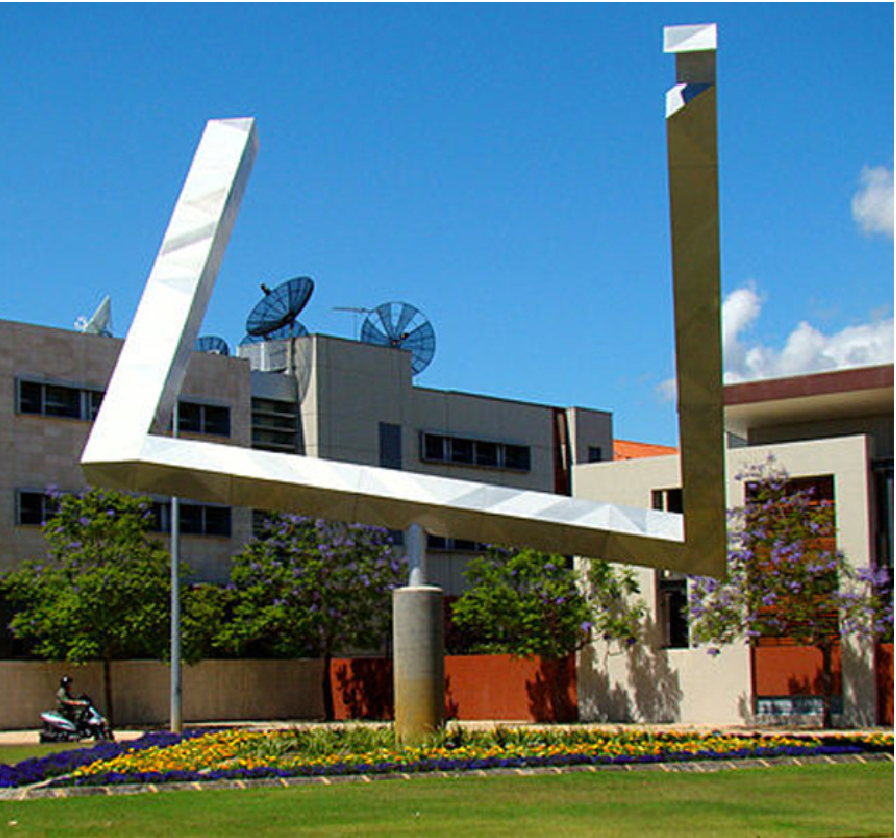
\includegraphics[height=4cm]{Penrose1} \qquad 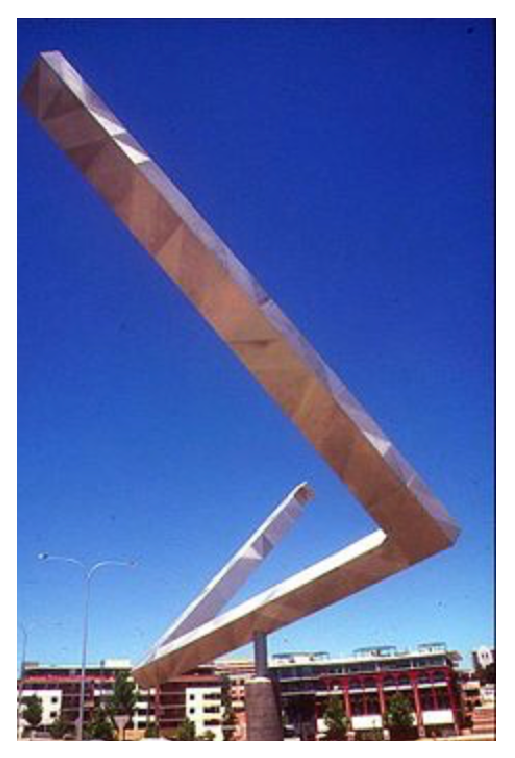
\includegraphics[height=4cm]{Penrose2} \qquad 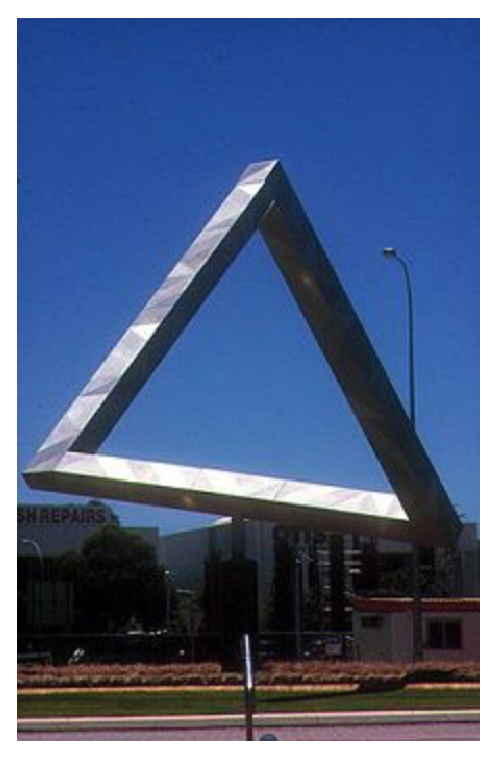
\includegraphics[height=4cm]{Penrose3}
\end{center}

\end{enigme}

